\chapter{Casistica, materiali e metodi}

\section{Casistica}

Introduzione alle informazioni della mostrate

\clearpage

\subsection{Paziente 1} % Ma.Va.

Breve descrizione ...
Sed ut perspiciatis unde omnis iste natus error sit voluptatem accusantium doloremque laudantium, totam rem aperiam, eaque ipsa quae ab illo inventore veritatis et quasi architecto beatae vitae dicta sunt explicabo. Nemo enim ipsam voluptatem quia voluptas sit aspernatur aut odit aut fugit, sed quia consequuntur magni dolores eos qui ratione voluptatem sequi nesciunt. 

\begin{table}[!h]
\begin{tabular}{lrllrl}
\toprule
\multicolumn{6}{l}{\textbf{Dati alla nascita}}\\
Luogo 		& \multicolumn{2}{l}{Torino} 	& Data 					& \multicolumn{2}{l}{28/12/89} 	\\
Sesso 		& \multicolumn{2}{l}{Femmina} 	& Età gestazionale 		& 40 		& sett.\\
Lunghezza 	& 45 		& cm 					& Circonferenza cranica	& 35 		& cm\\
Peso 		& 3350 		& g\\
\midrule
\multicolumn{6}{l}{\textbf{Statura dei genitori}}\\
Padre 		& 165.5 & cm 	& Madre 				& 164.2 & cm \\
MPH 		& ?? 	& cm \\
\midrule
\multicolumn{6}{l}{\textbf{Trattamento con GH}} \\
Età	iniziale	& ?? & 		& Altezza iniziale 				& 135.5 & cm  \\
Peso iniziale	& 25.4 & kg	& Velocità di crescita iniziale & 4.13 & cm/aa\\
Dose media		& ?? & unità & Anni prepuberali trattati		& ??\\
Anni di terapia & ??\\
\midrule
\multicolumn{6}{l}{\textbf{Esito della terapia}} \\
Altezza finale	& ?? & cm 	& SDS guadagnate 			& ??\\
SDS per MPH		& ?? &		& SDS guadagnate per MPH	& ??
\bottomrule
\end{tabular}
\end{table}
\clearpage

\subsection{Paziente 2}

Sed ut perspiciatis unde omnis iste natus error sit voluptatem accusantium doloremque laudantium, totam rem aperiam, eaque ipsa quae ab illo inventore veritatis et quasi architecto beatae vitae dicta sunt explicabo. Nemo enim ipsam voluptatem quia voluptas sit aspernatur aut odit aut fugit, sed quia consequuntur magni dolores eos qui ratione voluptatem sequi nesciunt. Neque porro quisquam est, qui dolorem ipsum quia dolor sit amet, consectetur, adipisci velit, sed quia non numquam eius modi tempora incidunt ut labore et dolore magnam aliquam quaerat voluptatem. Ut enim ad minima veniam, quis nostrum exercitationem ullam corporis suscipit laboriosam, nisi ut aliquid ex ea commodi consequatur? Quis autem vel eum iure reprehenderit qui in ea voluptate velit esse quam nihil molestiae consequatur, vel illum qui dolorem eum fugiat quo voluptas nulla pariatur?

\begin{table}[!h]
\begin{tabular}{lrllrl}
\toprule
\multicolumn{6}{l}{\textbf{Dati alla nascita}}\\
Luogo 		& \multicolumn{2}{l}{Torino} 	& Data 					& \multicolumn{2}{l}{28/12/89} 	\\
Sesso 		& \multicolumn{2}{l}{Femmina} 	& Età gestazionale 		& 40 		& sett.\\
Lunghezza 	& 45 		& cm 					& Circonferenza cranica	& 35 		& cm\\
Peso 		& 3350 		& g\\
\midrule
\multicolumn{6}{l}{\textbf{Statura dei genitori}}\\
Padre 		& 165.5 & cm 	& Madre 				& 164.2 & cm \\
MPH 		& ?? 	& cm \\
\midrule
\multicolumn{6}{l}{\textbf{Trattamento con GH}} \\
Età	iniziale	& ?? & 		& Altezza iniziale 				& 135.5 & cm  \\
Peso iniziale	& 25.4 & kg	& Velocità di crescita iniziale & 4.13 & cm/aa\\
Dose media		& ?? & unità & Anni prepuberali trattati		& ??\\
Anni di terapia & ??\\
\midrule
\multicolumn{6}{l}{\textbf{Esito della terapia}} \\
Altezza finale	& ?? & cm 	& SDS guadagnate 			& ??\\
SDS per MPH		& ?? &		& SDS guadagnate per MPH	& ??
\bottomrule
\end{tabular}
\end{table}

\clearpage

\subsection{Paziente 3}

\clearpage

\section{Materiali e metodi}

\subsection{Valutazione auxologica}

\begin{figure}[h]
  \begin{center}
      \includegraphics{grafici/centili/centili.eps} %\\
  \end{center}
  \caption{Standard antropometrici neonatali relativi a peso ed altezza nell'Italia nord-orientale}
\end{figure}

\begin{figure}[h]
  \begin{center}
	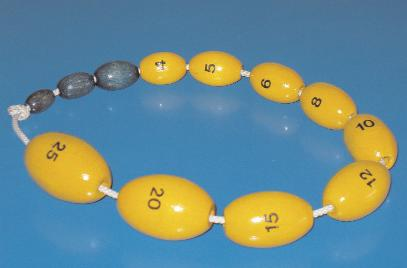
\includegraphics[scale=0.75]{grafici/orchidometro.jpg}
  \end{center}
  \caption{Orchidometro di Prader}
\end{figure}

\begin{figure}[h]
  \begin{center}
	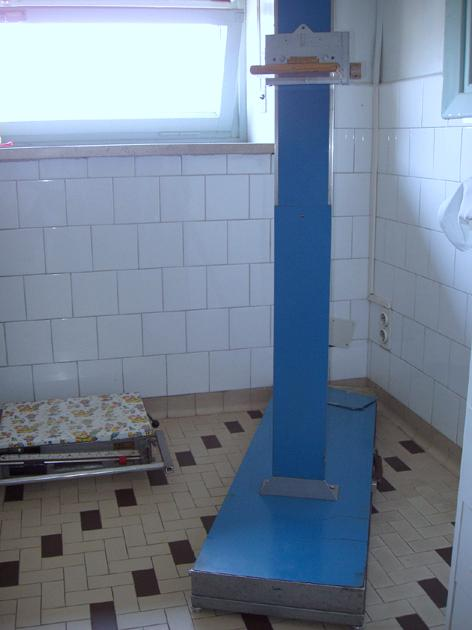
\includegraphics[scale=0.50]{grafici/statimetro.jpg}
  \end{center}
  \caption{Statimetro di Harpenden}
\end{figure}

\subsection{Valutazione ormonale}

\subsection{Analisi statistiche}
